\documentclass[tikz, border=5pt]{standalone}
\usepackage{pgfplots}
\pgfplotsset{compat=1.18}

% --- Definição das cores exatas baseadas na imagem ---
\definecolor{barOrange}{RGB}{253, 191, 87}
\definecolor{barBlue}{RGB}{201, 228, 238}
\definecolor{lineGreen}{RGB}{0, 128, 0}
\definecolor{gridGray}{RGB}{235, 235, 235}

\begin{document}

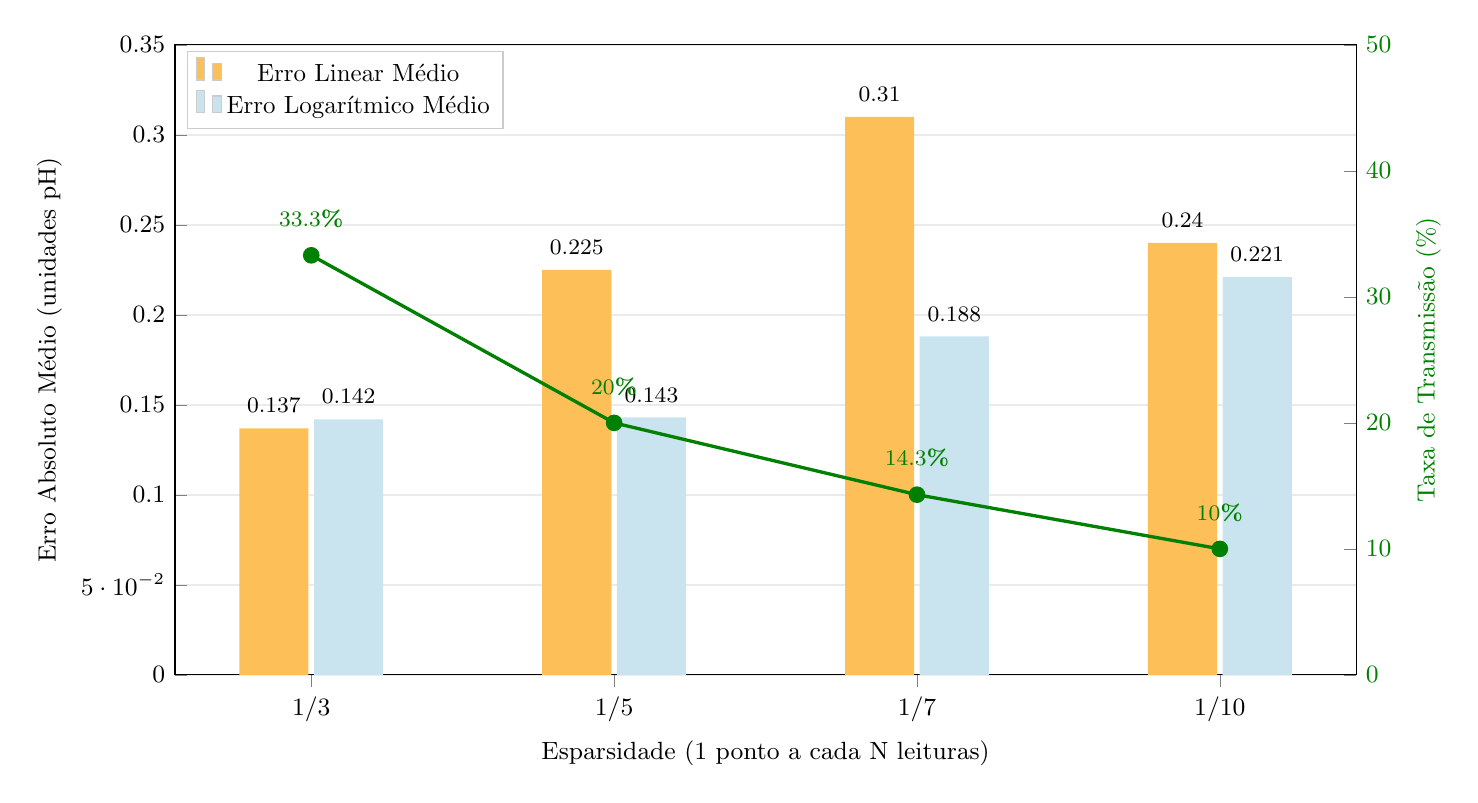
\begin{tikzpicture}
    % Configurações comuns de tamanho para garantir o alinhamento perfeito dos dois eixos
    \pgfplotsset{
        my graph size/.style={
            width=15cm,
            height=8cm,
            scale only axis, % Garante que width/height se aplicam exatamente à área de plotagem
            enlarge x limits=0.15, % Espaço nas laterais do eixo X para as barras não colarem na borda
        }
    }

    % ==================================================================
    % EIXO Y ESQUERDO (Gráfico de Barras)
    % ==================================================================
    \begin{axis}[
        my graph size,
        ybar, % Tipo de gráfico: barras agrupadas
        bar width=25pt, % Largura das barras
        % --- Configuração dos Eixos e Ticks ---
        ylabel={Erro Absoluto Médio (unidades pH)},
        xlabel={Esparsidade (1 ponto a cada N leituras)},
        symbolic x coords={1/3, 1/5, 1/7, 1/10}, % Rótulos textuais do eixo X
        xtick=data, % Mostra os tiques apenas onde há dados definidos
        xtick pos=bottom, % Ticks apenas embaixo
        ytick pos=left,   % Ticks apenas na esquerda
        ymin=0, ymax=0.35, % Limites do eixo Y esquerdo para acomodar os rótulos acima das barras
        ytick distance=0.05, % Intervalo dos tiques no eixo Y
        % --- Configuração da Grade ---
        ymajorgrids=true, % Ativa a grade horizontal
        grid style={gridGray, thick}, % Estilo da grade
        axis on top=false, % Garante que a grade fique atrás das barras
        % --- Configuração da Legenda ---
        legend style={
            at={(0.01,0.99)}, 
            anchor=north west, 
            nodes={scale=0.9, transform shape},
            draw=gray!40,
            % Código para criar o 'box' colorido na legenda
            legend image code/.code={%
                \draw[##1, draw=none, fill=##1] (0cm,-0.1cm) rectangle (0.3cm,0.1cm);
            }
        },
        % --- Configuração dos Rótulos de Valor (Numbers above bars) ---
        nodes near coords,
        every node near coord/.append style={
            font=\footnotesize,
            yshift=2pt, % Levanta um pouco o número para não colar na barra
            /pgf/number format/fixed,
            /pgf/number format/precision=3 % Força exatamente 3 casas decimais
        },
        % --- Estilos de Fonte ---
        tick label style={font=\small},
        label style={font=\small},
    ]

    % Dados Série 1: Erro Linear Médio (Laranja)
    \addplot[fill=barOrange, draw=none] coordinates {
        (1/3, 0.137)
        (1/5, 0.225)
        (1/7, 0.310)
        (1/10, 0.240)
    };

    % Dados Série 2: Erro Logarítmico Médio (Azul Claro)
    \addplot[fill=barBlue, draw=none] coordinates {
        (1/3, 0.142)
        (1/5, 0.143)
        (1/7, 0.188)
        (1/10, 0.221)
    };

    \legend{Erro Linear Médio, Erro Logarítmico Médio}
    \end{axis}

    % ==================================================================
    % EIXO Y DIREITO (Gráfico de Linha)
    % ==================================================================
    \begin{axis}[
        my graph size,
        axis y line*=right, % Eixo Y apenas na direita. O '*' evita que ele desenhe uma nova caixa de eixo sobre a anterior.
        axis x line=none,   % Esconde o eixo X (já mostrado pelo primeiro gráfico)
        % --- Configuração do Eixo Y Direito ---
        ylabel={Taxa de Transmissão (\%)},
        ymin=0, ymax=50, % Limites exatos do eixo Y direito conforme a imagem
        ytick distance=10,
        % Necessário repetir as coordenadas simbólicas para o alinhamento funcionar
        symbolic x coords={1/3, 1/5, 1/7, 1/10},
        xtick=data,
        % --- Estilização do Rótulo do Eixo Direito ---
        ylabel style={
            font=\small, 
            color=lineGreen,
            % Posicionamento manual para centralizar verticalmente ao lado do eixo
            at={(axis description cs:1.08,0.5)}, 
            anchor=south, 
            rotate=0    % [CORREÇÃO] Rotaciona 90 graus no sentido anti-horário (padrão de leitura)
        },
        yticklabel style={font=\small, color=lineGreen},
    ]

    % Dados Série 3: Taxa de Transmissão (Linha Verde)
    \addplot[
        lineGreen,
        very thick, % Linha mais grossa
        mark=*, % Marcador de círculo preenchido
        mark options={scale=1.2, fill=lineGreen}, % Tamanho e cor do marcador
        % --- Configuração dos Rótulos de Valor da Linha ---
        nodes near coords={%
            % Imprime o número com 1 casa decimal e adiciona o símbolo %
            \pgfmathprintnumber[fixed, precision=1]{\pgfplotspointmeta}\%%
        },
        every node near coord/.append style={
            font=\footnotesize\bfseries, % Fonte menor e negrito
            color=lineGreen,
            anchor=south, % Posiciona acima do ponto
            yshift=6pt    % Distância vertical do ponto
        },
    ] coordinates {
        (1/3, 33.3)
        (1/5, 20.0)
        (1/7, 14.3)
        (1/10, 10.0)
    };
    
    \end{axis}
\end{tikzpicture}

\end{document}